\documentclass[crop=false, class=memoir]{standalone}

\usepackage[utf8]{inputenc}%Nødvendig for danske bogstaver
\usepackage[danish]{babel}%Sørger for at ting LaTeX gør automatisk er på dansk
\usepackage{csquotes}
\usepackage{geometry}%Til opsætning af siden
\geometry{lmargin = 2.5cm,rmargin = 2.5cm}%sætter begge magner
\usepackage{lipsum}%Fyldtekst, til brug under test af layoutet
\usepackage{float}
\usepackage{graphicx}%Tillader grafik
\usepackage{epstopdf}%Tillader eps filer
\usepackage{marginnote}% Noter i margen
\interfootnotelinepenalty=10000 %undgår at fodnoter bliver spilittet op.
\usepackage[sorting=none]{biblatex}
\addbibresource{litteratur.bib}
\usepackage[hidelinks]{hyperref}%Tillader links
\usepackage{subcaption} % Tillader underfigurer
\usepackage[font={small,sl}]{caption}	% Caption med skrå tekst ikke kursiv

\usepackage{xcolor} %Bruges til farver
\usepackage{forloop} %Bruges til nemmere for loops

\newcounter{opgave}[chapter] %Definerer opgavenumrene og hvornår de nulstilles
\renewcommand{\theopgave}{\thechapter.\arabic{opgave}} %Definerer udseende af opgavenummereringen
\newcounter{delopgave}[opgave] %Definerer delopgavenumrene
\newcounter{lvl} %Definerer en "variabel" til senere brug

\definecolor{markerColor}{rgb}{0.0745098039, 0.262745098, 0.584313725} %Definerer farven af markøren
\newcommand{\markerSymbol}{\ensuremath{\bullet}} %Definerer tegnet for markøren
\newlength{\markerLength} %Definerer en ny længde
\settowidth{\markerLength}{\markerSymbol} %Sætter den nye længde til bredden af markøren

\newenvironment{opgave}[2][0]{%Definerer det nye enviroment, hvor sværhedsgraden er den første parameter med en default på 0
\newcommand{\opg}{\refstepcounter{delopgave}\par\vspace{0.1cm}\noindent\textbf{\thedelopgave)\space}}%Definerer kommando til delopgave
\refstepcounter{opgave}%Forøger opgavenummer med 1 og gør den mulig at referere til
\setcounter{lvl}{#1}%Sætter "variablen" lvl lig med angivelsen af sværhedsgraden
\noindent\hspace*{-0.75em}\hspace*{-\value{lvl}\markerLength}\forloop{lvl}{0}{\value{lvl}<#1}{{\color{markerColor}\markerSymbol}}\hspace*{0.75em}%Sætter et antal af markører svarende til sværhedsgraden
\textbf{Opgave \theopgave : #2}\newline\nopagebreak\ignorespaces}{\bigskip} %Angiver udseende af titlen på opgaverne samt mellemrummet mellem opgaver



\usepackage{mathtools}%Værktøjer til at skrive ligninger
\renewcommand{\phi}{\varphi}%Vi bruger varphi
\renewcommand{\epsilon}{\varepsilon}%Vi bruger varepsilon
\usepackage{physics}%En samling matematikmakroer til brug i fysiske ligninger
\usepackage{braket}%Simplere kommandoer til bra-ket-notation
\usepackage{siunitx}%Pakke der håndterer SI enheder godt
\DeclareSIUnit\clight{\text{\ensuremath{c}}} % Lysets fart i vakuum som c og ikke c_0
\usepackage{chemmacros}
\usechemmodule{isotopes}
\usepackage{tikz}
\usepackage[danish]{cleveref}
\usepackage{nicefrac}
% \renewcommand{\ref}[1]{\cref{#1}}
\creflabelformat{equation}{#2(#1)#3}
\crefrangelabelformat{equation}{#3(#1)#4 to #5(#2)#6}
\crefname{equation}{ligning}{ligningerne}
\Crefname{equation}{Ligning}{Ligningerne}
\crefname{section}{afsnit}{afsnitene}
\Crefname{section}{Afsnit}{Afsnitene}
\crefname{figure}{figur}{figurene}
\Crefname{figure}{Figur}{Figurene}
\crefname{table}{tabel}{tabellerne}
\Crefname{table}{Tabel}{Tabellerne}
\crefname{opgave}{opgave}{opgaverne}
\Crefname{opgave}{Opgave}{Opgaverne}
\crefname{delopgave}{delopgave}{delopgaverne}
\Crefname{delopgave}{Delopgave}{Delopgaverne}

\newcommand{\eqbox}[1]{\begin{empheq}[box=\fbox]{align}
	\begin{split}
	#1
	\end{split}
\end{empheq}}

\newcommand{\kb}{\ensuremath{k_\textsc{b}}}

\DeclareSIUnit{\parsec}{pc}
\DeclareSIUnit{\lightyear}{ly}
\DeclareSIUnit{\astronomicalunit}{AU}
\DeclareSIUnit{\year}{yr}
\DeclareSIUnit{\solarmass}{M_\odot}
\DeclareSIUnit{\solarradius}{R_\odot}
\DeclareSIUnit{\solarluminosity}{L_\odot}
\DeclareSIUnit{\solartemperature}{T_\odot}
\DeclareSIUnit{\earthmass}{M_\oplus}
\DeclareSIUnit{\earthradius}{R_\oplus}
\DeclareSIUnit{\jupitermass}{M_J}

% Infobokse og lignende
% http://mirrors.dotsrc.org/ctan/graphics/awesomebox/awesomebox.pdf
% \usepackage{awesomebox}


% Egen infobokse (virker kun med begrænsede symboler)

\usepackage[framemethod=tikz]{mdframed}
\usetikzlibrary{calc}
\usepackage{kantlipsum}

\usepackage[tikz]{bclogo}

\tikzset{
    % lampsymbol/.style={scale=2,overlay}
    % lampsymbol/.pic={\centering\tikz[scale=5]\node[scale=10,rotate=30]{\bclampe}}.style={scale=2,overlay}
    infosymbol/.style={scale=2,overlay}
}

\newmdenv[
    hidealllines=true,
    nobreak,
    middlelinewidth=.8pt,
    backgroundcolor=blue!10,
    frametitlefont=\bfseries,
    leftmargin=.3cm, rightmargin=.3cm, innerleftmargin=2cm,
    roundcorner=5pt,
    % skipabove=\topsep,skipbelow=\topsep,
    singleextra={\path let \p1=(P), \p2=(O) in ($(\x2,0)+0.92*(1.1,\y1)$) node[infosymbol] {\bcinfo};},
    % singleextra={\path let \p1=(P), \p2=(O) in ($(\x2,0)+0.5*(2,\y1)$) node[infosymbol] {\bcinfo};},
]{info}

% Skal bruges som
% \begin{info}[frametitle={Titel}]
%     Tekst
% \end{info}

\begin{document}

\chapter{Kosmologi} \label{chap:kosmo}
\section{Introduktion}
Kosmologi er læren om universets dannelse, udvikling og endeligt. Når der snakkes om universets størrelse, er det normalt det synlige univers, der menes. Dette er den del af universet, hvor lys er nået hen til os, så vi kan observere det. Længere ude er informationen ikke nået frem til os endnu, så vi ved ikke, hvor stort hele universet er. 

Det stemmer overens med \emph{det kosmologiske princip}, der siger, at universets love og konstanter er ens overalt, samt at massen er ligeligt fordelt (set fra en stor nok skala). Det kan deles op i to postulater: Universet er homogent (ens i hvert område man vælger) og isotropt (ser ens ud, uanset hvilken retning man kigger i), som illustreret i \cref{kosmo:fig:isohomo}. Det kosmologiske princip behøver ikke gælde, men vi har ikke tydeligt observeret noget, der bryder med det\footnote{Nogle mener at have observeret brud, men der er ikke enighed om det endnu.}. Princippet antages derfor normalt at gælde, da det er det simpleste -- vi har ingen grund til at tro, at universets egenskaber pludselig ændrer sig et sted. Det er en god approksimation på skalaer fra \SI{200}{\mega\parsec} (megaparsec) og opefter. \SI{1}{\parsec} er cirka 3 lysår, og et lysår (forkortet ly) er afstanden lys tilbagelægger på et år i vakuum: %$3\cdot 10^8$ lysår
\SI{2.8e13}{\kilo\metre}. Således er $\SI{200}{\mega\parsec} \approx \SI{6e8}{\lightyear} \approx \SI{6e21}{\kilo\metre}$.
På små skalaer holder det selvfølgelig ikke. For eksempel er du tættere (har større massefylde) end luften omkring dig, og Solen kan udpege en særlig retning inden for solsystemet (den er speciel i forhold til planeterne, så en bevægelse ind mod den er speciel).

\begin{figure}
	\centering
	%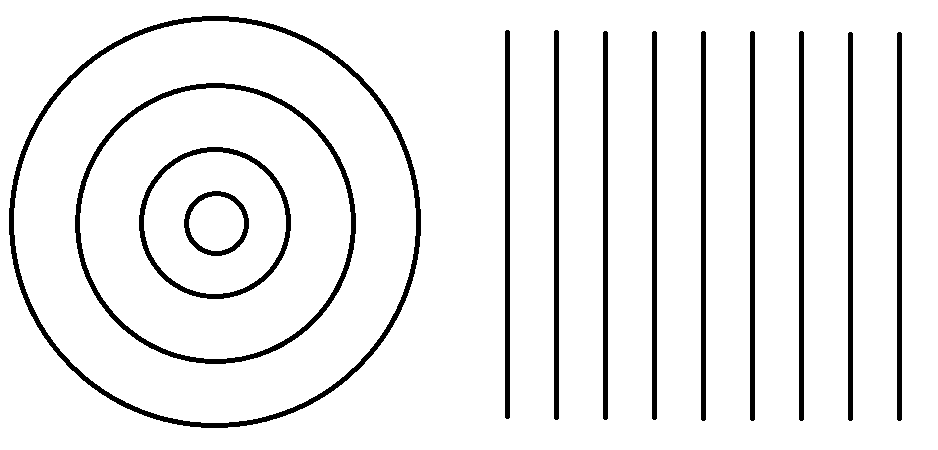
\includegraphics[width=0.7\textwidth]{Kosmo/img/isohomo.png}
	\begin{tikzpicture}[]
    \foreach \radius in {0.5, 1, 1.5, 2}
        \draw[ultra thick] (-2.5,0) circle (\radius cm);
    
    \foreach \radius in {0.5, 1, 1.5, 2, 2.5, 3, 3.5, 4, 4.5}
        \draw[ultra thick] (0.5+\radius,-2) -- ++(0,4);
    \end{tikzpicture} 
	\caption{Venstre: Illustration af isotropi. Fra midten ser verden ens ud i alle retninger. Højre: Illustration af homogenitet. Kigger man på et stort nok udsnit af verden, vil det se ud som alle andre udsnit.}
	\label{kosmo:fig:isohomo}
\end{figure}

Antagelsen om, at universet er homogent og isotropt, er understøttet af kortlægningen af den \emph{kosmiske mikrobølgebaggrund} (engelsk: CMB – Cosmic Microwave Background). Baggrunden består af stråling fra det tidspunkt, hvor universet blev gennemsigtigt (ca. 380.000 år efter Big Bang) –- altså hvor temperaturen af det plasma og stråling, som var dannet efter Big Bang, er aftaget så tilstrækkeligt, at det var muligt for frie elektroner at binde sig til atomkerner og danne hydrogen og helium, hvormed lys pludselig kunne bevæge sig næsten frit, og derved undslippe. Af historiske årsager kaldes det \emph{rekombinationen}, da de første atomer dannes. At fotonerne derfor kunne bevæge sig frit kaldes \emph{fotonafkoblingen}, og disse to begivenheder skete næsten samtidig. Den kosmiske mikrobølgebaggrund er derfor det ældste lys i universet! Dengang var strålingen i UV-området\footnote{Det vil sige med en bølgelængde fra omkring \SI{10}{\nano\metre} til omkring \SI{400}{\nano\metre}, hvilket er kortere end synligt lys.}, men udvidelsen af Universet (se \cref{kosmo:sec:roedforskydning}) har nu kølet baggrundsstrålingen til en temperatur på \SI{2.73}{\kelvin} eller \SI{-270.42}{\celsius} og flyttet den til mikrobølgeområdet\footnote{Det vil sige med en bølgelængde fra omkring \SI{1}{\milli\metre} til omkring \SI{1}{\metre}, hvilket er meget længere end synligt lys.} (energi og temperatur er for stråling afhængige af hinanden). Den kosmiske mikrobølgebaggrund er blevet kortlagt af flere missioner, først COBE (Cosmic Background Explorer), siden WMAP (Wilkinson Microwave Anisotropy Probe) og senest \textit{Planck}, se \cref{kosmo:fig:CMB}. Det ses, at selv med høj opløsning er kortet uniformt – beviset på et næsten homogent og isotropt tidligt univers. Men små fluktuationer i tætheden er stadig til stede, og var det ikke for disse, ville den gravitationelle tiltrækning ikke have kunnet ført til de galakser, vi observerer (og bor i!) i dag.

\begin{figure}
	\centering
	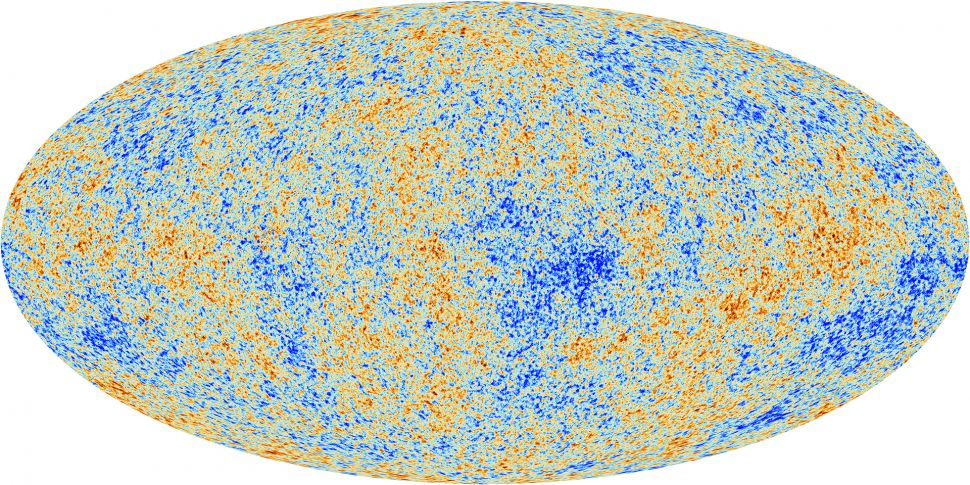
\includegraphics[width=0.65\textwidth]{Kosmo/img/cmb_planck.jpg}
	\caption{Kortlægningen af den kosmiske mikrobølgebaggrund af COBE, WMAP og
		Planck. Mælkevejen, som ellers ville være til stede i billedet, er redigeret ud. Farverne viser de bittesmå temperaturfluktuationer på \SI[detect-shape]{+-300}{\micro\kelvin}. Kilde:~\cite{CosmicMicrowaveBackground}.}%\textit{Billedekilde: ESA og the Planck Collaboration}}
	\label{kosmo:fig:CMB}
\end{figure}
%Fra http:
%		//www.planetastronomy.com/astronews/astrn-2013/04/astron3.jpg

%\section{Big Bang og CMB}
\section{Rødforskydning}\label{kosmo:sec:roedforskydning}
\subsection{Dopplerforskydning}
Du kender nok til, at når en ambulance kører forbi, så lyder sirenens tone højere, når ambulancen nærmer sig, og dybere når den kører væk. Det skyldes \emph{Dopplerforskydning}, %Find gerne lydklip til undervisningen
%Det skyldes, 
hvilket er at lydbølgerne skubbes sammen og strækkes, afhængigt af hvilken fart de udsendes med i forhold til lytteren. Hvis en ambulance kører mod dig, og du står stille, vil du høre bølgerne sammenpresset. Dette skyldes, at lydens hastighed er uændret i mediet. Lydbølgen bliver udsendt under bevægelse, dvs. at i det tidsrum bølgen bliver sendt ud over, så flytter ambulancen sig også. Derfor vil bølgen virke til at have en kortere bølgelængde, da afstanden har ændret sig under udsendelse (se \cref{kosmo:fig:doppler}). %\\
Men hvis du selv kører med samme hastighed foran ambulancen, så vil du høre dem på samme måde, som de bliver udsendt -- altså på samme måde, som hvis begge biler står stille, da det er den relative hastighed, som er afgørende.

\begin{figure}
	\centering
	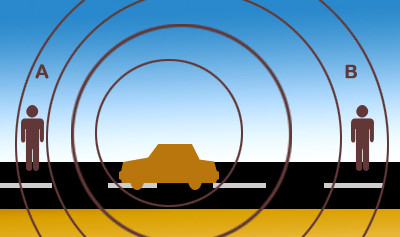
\includegraphics[width=0.55\textwidth]{Kosmo/img/doppler.jpg}
	\caption{Dopplerforskydning af lyden fra en bil, der kører mod venstre. Person A vil høre end højere tone end person B, og personen i bilen vil høre noget et sted derimellem. Ringene viser et fast punkt på lydbølgerne. Kilde: \cite{DopplerIllustration}.}
	\label{kosmo:fig:doppler} 
\end{figure}

Det samme sker for lys. Hvis en ambulance kører væk, vil både tonen af sirenen blive dybere og lyset fra lygterne en smule rødere. Med rødere menes her, at lyset forskydes til at få en længere bølgelængde, og da rødt lys er den del af det visuelle spektrum, der har længst bølgelængder, så vil visuelt lys se rødere ud. Man kalder det derfor også rødforskydning generelt.

Bemærk dog, at selvom fotoner og lydbølger har højere energi ved korte bølgelængder, så mister de ikke energi ved Dopplerforskydning -- der er bare sket et skift i perspektivet, man ser bølgerne fra. Fra bølgens eget synspunkt (hvis man følger den), har den samme bølgelængde og energi hele tiden\footnote{Sådanne tanker om hvordan ens bevægelse påvirker, hvordan man opfatter verden, er helt central for speciel og generel relativitetsteori. Mere om det i \cref{chap:rel}.}.

\subsection{Kosmologisk Rødforskydning}
Edwin Hubble er en kendt skikkelse, som i 1920'erne var involveret i opdagelsen af, at galakser langt borte ser rødforskudte ud, men dette skyldes \emph{ikke} Dopplerforskydning fra galaksernes egenhastighed\footnote{Egenhastighed vil sige den hastighed som galaksen ``selv'' oplever at den har.} i forhold til os. Så ville vi have forventet, at lige så mange galakser var rødforskudte som blåforskudte, hvis de starter med en tilfældig hastighed. Og det gør de jo -- for hvorfor skulle de alle have en særlig retning i forhold til os? Det ville bryde med isotropien. 

Hubble bemærkede, at galakserne oftere er rødforskudte end blåforskudte -- ja næsten altid rødforskydte -- og jo længere væk de er, desto mere rødforskudte er de også. Georges Lemaître havde dog allerede formuleret og observeret, hvad der nu kaldes \emph{Hubble–Lemaîtres lov} (tidligere kendt som Hubbles lov), der beskriver den direkte proportionalitet mellem afstand og fart af en galakse (hvortil Hubble bidrog med mere data),
%
\begin{align}
    v=H_0 D, \label{kosmo:eq:Hubbleslaw}    
\end{align}
%
hvor $v$ er farten væk fra os, $D$ er afstanden til galaksen, og $H_0$ er Hubbles konstant, som er den nuværende værdi af Hubbleparameteren (der ikke er konstant, men ændrer sig meget langsomt). Det er desværre vanskeligt at sige præcis, hvad værdien af Hubblekonstanten er, da forskellige typer data, giver forskellige resultater. Dette er naturligvis interessant, og et af de mysterier astrofysikere lige nu arbejder på at løse. Værdien lader i hvert fald til at ligge omkring $\SI{70}{\kilo\meter\per\second\per\mega\parsec}$; et af budene er $H_0 = \SI{67.7+-0.5}{\kilo\meter\per\second\per\mega\parsec}$ \cite{planck}.

%Nævn de primære metoder, der bliver til at måle Hubblekonstanten.

Galaksers relative hastighed til os er altså større, desto længere væk de er. Og sådan vil det se ud fra ethvert punkt i universet. Derfor må rødforskydningen stamme fra, at alting bevæger sig længere væk fra hinanden, som rosiner i en hævende bolle. Det er netop, hvad der sker -- universets `dej' dvs. selve rumtiden\footnote{Begrebet rumtid kommer af, at man i relativitetsteori betragter rum og tid som værende to sider af samme sag. Man siger, at verden eksisterer i tre rumlige og en tidslig dimension, hvor de fire dimensioner tilsammen udgør rumtiden. For mere information se \cref{chap:rel}.} `hæver'. Galakserne har lige ofte egenhastigheder, der går mod os, som væk fra os, men hastigheden, som selve rumtiden udvider sig med, er vigtigere for galakser langt væk, fordi der er så meget rum imellem dem og os. For fjerne galakser skal lyset bevæge sig gennem mere rum, for at nå frem til os. Derfor når lyset at blive strukket mere end ved nære galakser, da rummet når at udvide sig mere under lysets rejse, og bølgelængden når således at blive strukket mere.

Ved rødforskydning fra universets udvidelse mister lyset rent faktisk energi i modsætning til almindelig Dopplerforskydning. Dette er selvfølgelig et brud på energibevarelse, men det er egentlig ikke et problem, da man ikke kan betragte universet som et lukket system, fordi det udvider sig. Energibevarelse behøver kun at gælde i lukkede systemer. Nogle mener dog, at ændringen i energi fra universets udvidelse (og den mørke energi, der opstår, se \cref{kosmo:sec:bestanddele}) udlignes af, at den gravitationelle energi falder til endnu lavere negative niveauer, således at universets totale energi altid er 0.

Måden, man måler rødforskydningen på, er ved at opsplitte lyset i dets forskellige bølgelængder. Dvs. man tager spektre af fjerne objekter, og derefter genkender man mønstre fra laboratorier på Jorden. Niels Bohr fik ideen, at elektroner kun kan eksistere i bestemte baner om en atomkerne, men ikke mellem disse. Hver bane har en bestemt energi, så elektronernes energi i atomer er kvantiseret, dvs. de kan kun have den energi, der svarer til lige præcis banernes energier. %findes kun i bestemte pakker. 
Når en elektron henfalder til en lavere tilstand, kommer den af med overskydende energi, ved at udsende en foton -- en lyspartikel. Hvis en foton med passende energi rammer en elektron, kan fotonen blive absorberet, så elektronen kommer op i en højere energitilstand\footnote{Denne måde at beskrive lys og atomer på er kvantemekanik, og sprogbruget, så som ``lyspartikel'' eller ``lyskvant'', kommer derfra.}. 

\begin{figure}[]
	\centering
	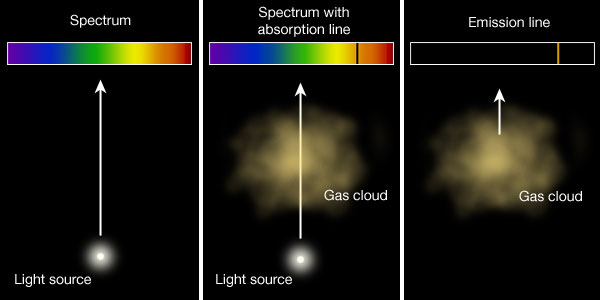
\includegraphics[width=0.6\textwidth]{Kosmo/img/kirchoffslaws.jpg}
	\caption{Kontinuert spektrum (til venstre), absorptions-spektrum (midtfor) og emissions-spektrum (til højre). Selve spektret er de farvede bånd øverst i figuren, som viser hvilke farver, der når frem til os. Absorptionslinjer er derfor manglen på bestemte farver i spektret, mens emissionslinjer er tilstedeværelsen af helt specifikke farver, hvor der ikke er nogle farver imellem. Kilde: \cite{AbsorptionEmissionSpectra}.}
	\label{kosmo:fig:kirchoff}
\end{figure}
%fra http://astro.psu.edu/public-outreach/fireworks-masks-1/absorption-and-emission-spectra

For lysspektrer gælder 3 love, kaldet Kirchoffs love (ikke at forveksle med Kirchoffs love for elektriske kredsløb), som er illustreret i \cref{kosmo:fig:kirchoff}.
\begin{itemize}
	\item Varme, uigennemsigtige objekter udsender lys kontinuert over hele spektret. Ideelt set ville det give spektret for sortlegemestråling, og det er en særligt god approksimation for varme stjerner. Sortlegemestråling er almindelig stråling som følge af, at objektet er varmt. Dette beskrives ved en lyskurve, under navnet Planckkurven, som er afhængig af objektets overfladetemperatur. Mindre stjernes lys er mere `forurenet' af effekter fra molekylær hydrogen, der er relativt koldt, samt andre grundstoffer og kemiske forbindelser.
	\item Varme, gennemsigte gasser udsender lys (da elektroner exciteres og henfalder) og danner emissionsspektra.
	\item Kolde gasser danner absorptionslinjer. Hvis en stjerne ligger bagved og sender lys mod os, vil skyen absorbere lyset og udsende det senere i en tilfældig retning. Dette betyder i længden, at det vil sende lys ud jævnt i alle retninger, hvilket giver en kraftig reduktion i mængden af lys der når os, da alt lyset pludselig skal fordeles i alle retninger. Så derfor ser vi mindre lys ved denne bølgelængde, end hvis gassen ikke havde været der.
\end{itemize}

\begin{figure}[]
	\centering
	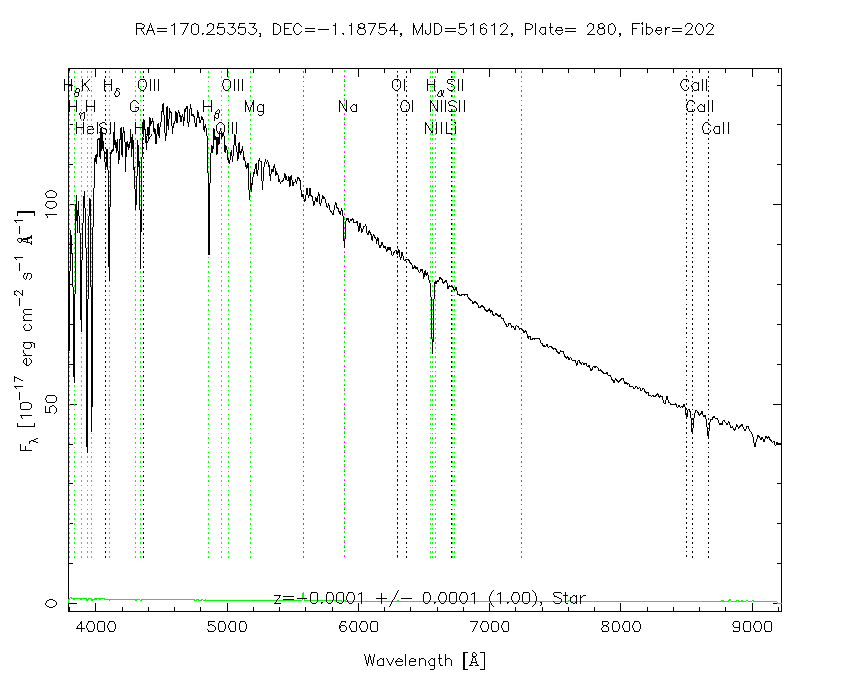
\includegraphics[width=0.6\textwidth]{Kosmo/img/spektrum.png}
	\caption{Et typisk stjernespektrum. $y$-aksen viser lysstyrken som flux (se \cref{kosmo:eq:flux}), mens der på $x$-aksen er bølgelængde i Ångstrøm (\si{\angstrom}) ($\SI{1}{\angstrom} = \SI{e-10}{\meter}$). Dykkene i intensitet er angivet med en overgang tilhørende et grundstof eller kemisk forbindelse, som er identificeret i stjernens atmosfære. Kilde:~\cite{Stjernespektrum}.}
	\label{kosmo:fig:spektrum}
\end{figure}
%fra http://i.stack.imgur.com/RMHmB.gif

Har man en galakse med en stjerne, som udsender et bredt spektrum af lys, vil lyset både bevæge sig gennem stjernens ydre `kolde' lag og galaksens gasskyer, før det når os. Stjerner og skyer består af forskellige stoffer såsom hydrogen. Når de belyses, absorberer hydrogenet fotoner med de energier, der svarer til energiforskellen mellem banerne i hydrogen. Der dannes derfor et helt bestemt mønster af absorbtionslinjer i spektret, som er unikt for i dette tilfælde hydrogen. For en rødforskudt galakse vil mønsteret ligge ved længere bølgelængder, end det vi måler for hydrogen på Jorden, men det er stadig genkendeligt, som det samme mønster. Et eksempel er vist i \cref{kosmo:fig:spektrum}. Når vi kan genkende et mønster af absorptionsliner eller emissionslinjer, selvom ligger forskudt ved andre bølgelængder end normalt, så kan vi bestemme et tal, der kvantificerer rødforskydningen. Dette tal, kaldet \emph{rødforskydningen}, er defineret som forskellen mellem den observeret bølgelængde, $\lambda_\textup{obs}$, og den i laboratoriet målte bølgelængde, $\lambda_\textup{lab}$, i forhold til laboratoriebølgelængden (se \cref{kosmo:fig:redshiftmeasure}). Det er altså den relative forskydning i forhold til den oprindelige bølge. Lad os opskrive det som
%
\begin{align}
    z &= \frac{\lambda_\textup{obs}-\lambda_\textup{lab}}{\lambda_\textup{lab}}. \label{kosmo:eq:redshifty}
    %
    \intertext{Rødforskydningen, $z$, er relateret til farten, $v$, således:}
    %
    z+1 &= \sqrt{\frac{1+v/c}{1-v/c}}. \label{kosmo:eq:redshift_velocity}
    %
    \intertext{For hastigheder meget langsommere end lysets hastighed i vakuum, $v \ll c$, kan det forsimples til:}
    %
    z &\approx \frac{v}{c}. \label{kosmo:eq:redshift_approx}
\end{align}
%
Rødforskydning er altså en form for afstandsmål (da farten, $v$, hænger sammen med afstanden, $D$, ifølge \cref{kosmo:eq:Hubbleslaw}), men også et tidsmål, da lyset har rejst i lang tid, hvis det har nået at passere en stor afstand, og er blevet strukket meget. Hvordan rødforskydningen relaterer til andre måder at måle afstand på, afhænger af hvordan rumtiden strækker lyset. Det kan afgøres af universets form via generel relativitetsteori.

\begin{figure}
	\centering
	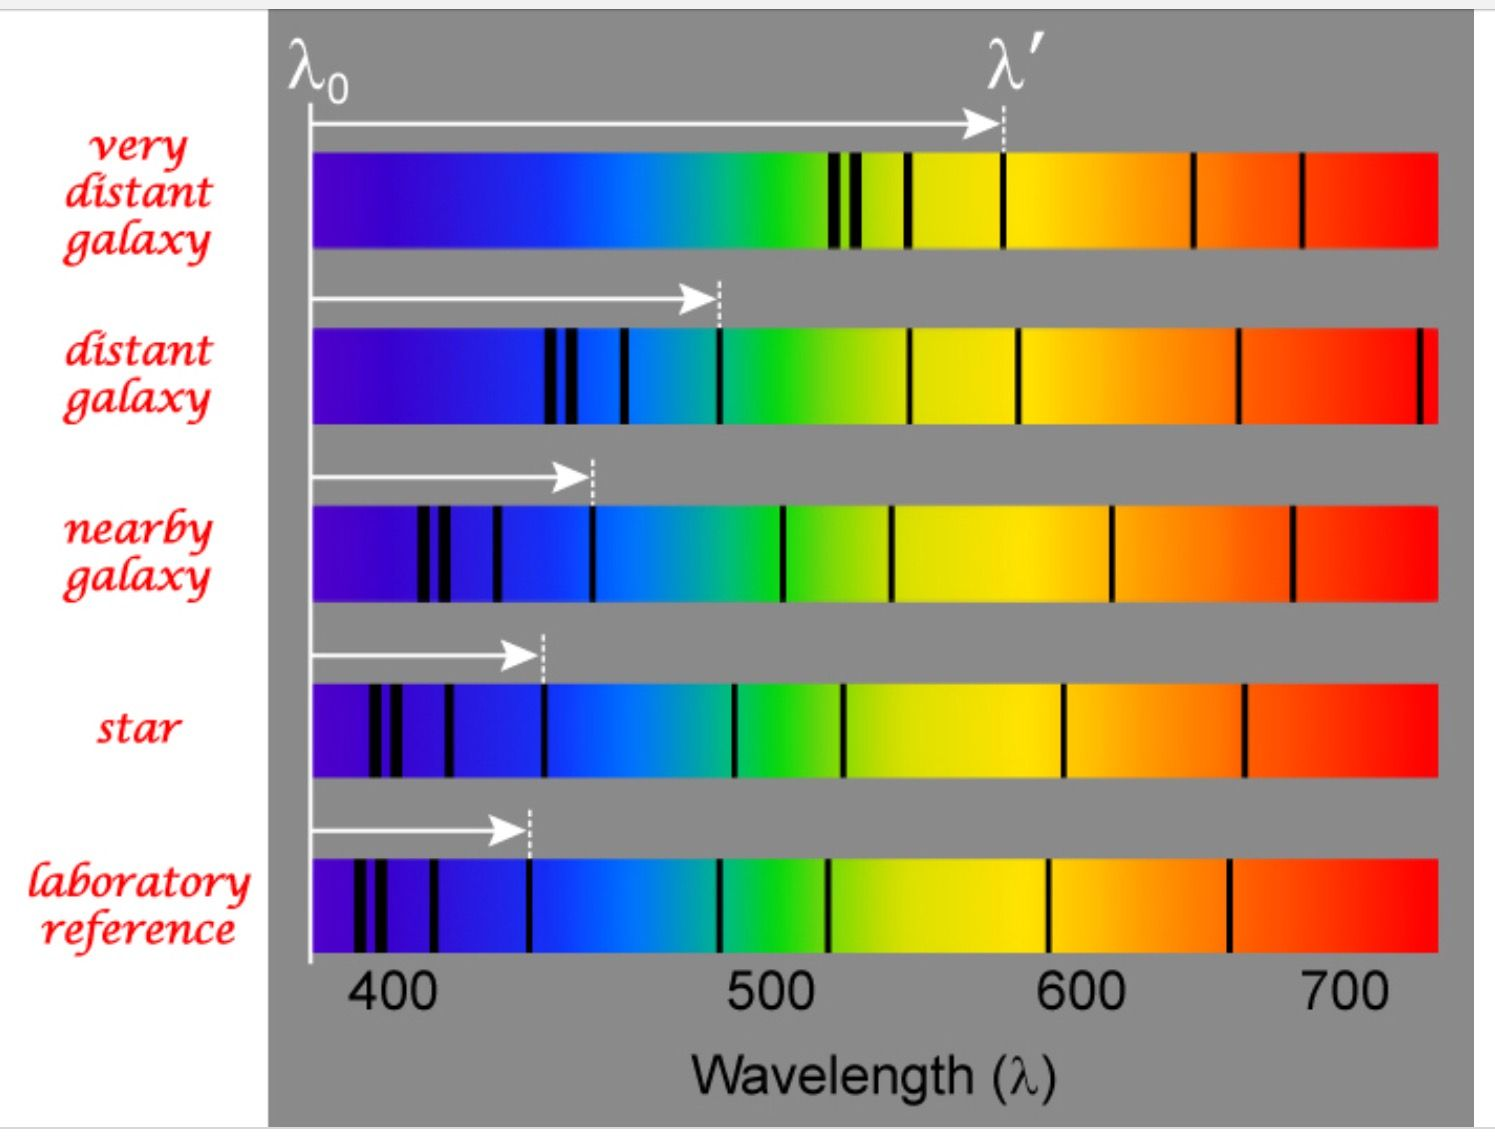
\includegraphics[width=0.55\textwidth]{Kosmo/img/redshiftcomparison.jpg}
	\caption{\Cref{kosmo:eq:redshifty} bruges ved at måle de indbyrdes forhold mellem absorptionslinjerne i de forskellige spektra. Vi kan se det samme mønster af sorte linjer (absorptions linjer) i hvert spektrum, men det er forskudt alt efter hvor langt lyskilden er væk. Kilde:~\cite{SNC1DEarthSpace}.}
	\label{kosmo:fig:redshiftmeasure}
\end{figure}

\section{Universets Form}

Universet har samlet set en form. Vi har 3 tydelige rumlige dimensioner omkring os, og vi er vant til, at hvis man tegner to parallelle linjer, så vil de aldrig krydse, samt at en trekant har altid en vinkelsum på \SI{180}{\degree}. Dette gælder dog kun i fladt rum! Forestil dig f.eks. en trekant tegnet på en globus; den vil faktisk have en vinkelsum på mere end \SI{180}{\degree}. På samme måde vil en trekant tegnet på en saddel have en vinkelsum, der er mindre end \SI{180}{\degree}. Dette er illustreret i \cref{kosmo:fig:shapes}. Hvis universet er kugleformet, siges det geometrisk at have en positiv krumning, og hvis det er saddelformet (hyperbolsk), siges det geometrisk at have en negativ krumning\footnote{En saddelform er ikke en perfekt illustration, da den bryder det kosmologiske princip ved at have et specielt center. I virkeligheden kan et negativt krumt univers godt have samme form overalt.}. I et fladt univers er krumningen 0.

\begin{figure}[]
	\centering
	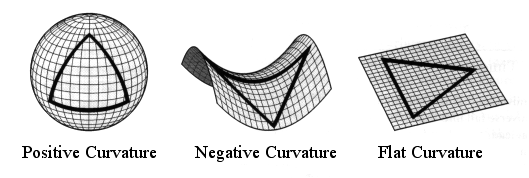
\includegraphics[width=0.75\textwidth]{Kosmo/img/universe_geometry.png}
	\caption{Trekanter i forskellige geometrier har forskellige vinkelsummer. Kilde:~\cite{GeometryUniverse}.}
	\label{kosmo:fig:shapes}
\end{figure}

Hvis en genstand er i frit fald, eller hvis man har en lysstråle, vil den bevæge sig langs en ret linje i rumtiden (kaldet en geodæt). Men hvis selve rumtiden krummer, så gør den `rette' linje det også. Derfor kan man se universets krumning ved at kigge på lyset fra objekter langt væk. Den viser sig ved, om ting ser forstørrede eller formindskede ud (om strålerne spredes eller samles som i en linse). Disse målinger viser, at universet er fladt med en præcision på \SI{0.5}{\percent}. Det vender vi tilbage til i \cref{kosmo:sec:bestanddele}. %Kilde + illustration

Hvis universet har en positiv krumning og er småt nok, så ville det også betyde, at lyset kunne nå hele vejen rundt, og vi ville se de samme objekter flere steder på himlen, hvilket heller ikke er observeret. Forestil dig, at du kaster en bold hårdt nok til, at den bevæger sig hele vejen rundt om jorden, og rammer dig i nakken igen. Det synlige univers er ser derfor meget fladt ud -- men måske har rumtiden en svag krumning, der bare ikke kan ses her. Selvom Danmark ser fladt ud, kan hele jordkloden godt være rund.

Hvis universet er positivt krumt, er det endeligt, mens fladt eller negativt krumt rum kan være uendeligt stort. Det er dog også muligt for universet både at være f.eks. fladt og endeligt, men så bryder man det kosmologiske princip: et fladt, endeligt rum har et centrum.

Vi kan sammenligne universets størrelse ved forskellige tidspunkter gennem en skalafaktor $a(t)$. Vi definerer den til at opfylde, at skalafaktoren i dag er 1, dvs. $a(t_0)=1$, hvor $t_0$ er tiden nu. Der gælder at
%
\begin{align}
    \frac{a(t_0)}{a(t)} &= 1+z, \\
    a(t) &= \frac{1}{1+z},
    %
    \intertext{hvor $z$ er rødforskydningen fra \cref{kosmo:eq:redshifty,kosmo:eq:redshift_velocity,kosmo:eq:redshift_approx}. Man kan derfor let omregne rødforskydning til skalafaktoren, fra dengang lyset blev udsendt.
    Som beskrevet % i \ref{Hubble}
    i forbindelse med \cref{kosmo:eq:Hubbleslaw}, er Hubblekonstanten ikke konstant, men blot den nuværende værdi af Hubbleparameteren. Hubbleparameteren er faktisk}
    %
    H &= \frac{v}{D} = \frac{\dot{a}}{a},
    %
    \intertext{hvor $\dot{a} = \dv*{a}{t}$, altså skalafaktoren differentiereret mht. tiden, eller den relative ændring i skalafaktoren. Hvis vi sætter det i anden og bruger noget generel relativitetsteori, som desværre er lidt for langhåret til at vi her vil vise det, får vi \emph{Friedmannligningen},}
    %
    H^2 = \left(\frac{\dot{a}}{a}\right)^2 &= \frac{8\pi G \rho}{3} - \frac{\kappa c^2}{a^2} + \frac{\Lambda}{3}, \label{kosmo:eq:friedmann}
\end{align}
%
hvor $\rho$ er densitet. Forklaring af de andre symboler følger. Hvis universet er fladt, må det have en helt bestemt samlet densitet kaldet den kritiske densitet $\rho_\textup{c} = \SI{8.6e-27}{\kilo\gram\per\cubic\metre}$. Friedmannligningen er superinteressant, da den viser os, hvordan universet udvikler sig. Det er en andenordensdifferentialligning med skalafaktoren $a$, der indeholder konstanter som gravitationskonstanten, $G$, og lysets fart i vakuum, $c$. $\kappa$ kan være 1, 0 og -1 og dette afgør krumningen, der som bekendt kan være positiv, flad eller negativ. $\Lambda$ (det store græske bogstav lambda) er den kosmologiske kontant. Uden denne ville rumtiden trække sig sammen, fordi massen krummer det. Einstein introducerede $\Lambda$ for at holde universet statisk, hvilket man dengang troede var sandt. Det har han senere kaldt sin største fejl, efter Hubble og Lemaître opdagede, at universet er dynamisk -- det ændrer sig med tiden. Man har dog genintroduceret konstanten for at accelerere udvidelsen, da man opdagede universets acceleration i 1998. Årsagen bag denne acceleration, er blevet tolket som en form for energi, kaldet \emph{mørk energi}. Lad os se på, hvad det egentlig er.

\section{Universets Komponenter}\label{kosmo:sec:bestanddele}
Universets udvikling og skæbne afhænger af dets indhold. Det består af:
%
\begin{itemize}
	\item Stråling/relativistisk stof: Fotoner og neutrinoer\footnote{En neutrino er en partikel, man arbejder med i partikelfysik, som ingen elektrisk ladning har. Derudover er dens masse meget lille. De to ting gør den meget svær at måle i eksperimenter. Den er vigtig i forbindelse med radioaktive betahendfald, for at opretholde bl.a. impuls- og energibevarelse.}, fordi de har ingen eller meget lav masse samt høj hastighed, hvilket betyder, at deres energi vil være domineret af kinetisk/relativistisk energi, og ikke deres masse (her menes hvilemasse).
	\item Stof: Almindeligt stof, antistof og mørkt stof har alle masse, så her kalder vi dem samlet set `stof'. Egenskaben masse afgør, hvor stor en kraft man skal bruge på at accelerere partiklerne, men også hvor meget de krummer rumtiden omkring sig. Stof kan også betegnes som `ikke-relativistisk' stof, dvs. stof der er domineret af masse, og ikke kinetisk energi. Det stof, der ikke er mørkt stof, kalder man nogle gange \textit{baryonisk}, da det mest består af baryoner. Baryoner er partikler med et ulige antal kvarker, fx. protoner\footnote{En proton består af to af de så kaldte op-kvarker og en ned-kvark. Kvarkerne navne kommer fra kvantemekanik, mere specifikt kvantefeltteori.} og neutroner\footnote{En neutron består af en af de så kaldte op-kvarker og to op-kvark.}.
	\item Kosmologisk konstant: Den form for mørk energi, vi antager universet er fyldt med. Det får universets udvidelse til at accelerere, er ligeligt fordelt overalt og fortyndes ikke fra udvidelsen. Det vides ikke om dette er en enkelt, samlet ting, eller en gruppe af ting (ligesom de ovenstående).
\end{itemize}
%
Disse komponenter påvirker universets form og udvikling forskelligt. Mængden af stof er nogenlunde konstant, men universet udvider sig i alle 3 rumlige dimensioner, så massedensiteten falder med:
%
\begin{align}
    \rho_\textup{m} &\propto a^{-3}.
    %
    \intertext{Tegnet $\propto$ betyder ``proportional med''.
    Stråling har næsten ingen \emph{hvilemasse}, hvilket er den masse et objekt har, når den står stille, men ved høj fart får de, hvad man kalder en relativistisk masse. Fotoner har jo energi, $E$, og impuls, $p$, og ifølge Einsteins ligning $E^2 = (mc^2)^2 + (pc)^2$ kan disse konverteres til masse, $m$, og derved vekselvirke via tyngdekraften med rumtiden. Det er derfor lys ikke kan undslippe sorte hullers masse, selvom lyset ikke har en hvilemasse. Denne `effektive masse' bøjer rummet omkring sig, så stråling får universet til at trække sig sammen, ligesom stof. Stråling har dog den ekstra egenskab, at den rødforskydes. Derfor fortyndes energien af stråling både med universets udvidelse, $a^{-3}$, og en ekstra faktor fra rødforskydningen, $a^{-1}$, fordi lys mister energi, når dets bølgelængde bliver større. Strålingstætheden skalerer således med skalafaktoren som}
    %
    \rho_\textup{R} &\propto a^{-4}.
    %
    \intertext{Mørk energi ved man ikke særlig meget om, men man formoder ofte, at det stammer fra energien i vakuum. Der er dog et ekstremt stort problem ved dette -- et bud på vakuumenergidensiteten fra kvantefeltteori\footnote{Kvantefeltteori er den bedste beskrivelse man har af universets mindste bestanddele, og bruges derfor i partikelfysik. I alle andre sammenhænge fungerer den rigtig godt, hvorfor dens bud på vakuumdensiteten er værd at bemærke. At kvantefeltteori giver en så forkert forudsigelse illustrerer et af de største uløste problemer i fysik: foreningen af kvantemekanik og generel relativitetsteori.} er $10^{124}$ gange større end universets kritiske energidensitet, $\rho_\textup{c}$ (se %\textit{Introduction to cosmology} af Barbara Ryden 
    \cite{rydenIntroductionCosmology2006})!  Det lader altså til den mest sandsynlige mængde energi i vakuum er alt for stor i forhold til vores observationer. Dette kan ses som et af mange usandsynlige tilfælde, der gør, at universet akkurat passer til, at liv kan opstå. Denne problemstilling er kendt som \emph{the finetuning problem}\footnote{Navnet kommer af spørgsmålet om, hvorfor de fysiske konstanter lige præcis har de værdier, de har. Hvis eksempelvis Plancks konstant var meget større, end den er, så ville vi se fænomener fra kvantemekanik i vores dagligdag. Ligeledes ville vi se effekter fra speciel og generel relativitetsteori, hvis lysets fart i vakuum var meget mindre end den er.}, og der er mange mulige løsninger på det. De er ofte ganske farverige, f.eks. multiverser, virtuelle universer og brud på det kosmologiske princip gennem variende konstanter på tværs af sted.\endgraf %\cite{TheAccUniverse} 
    I den simple antagelse, at mørk energi består af en ``kosmologisk konstant'', vil energien ikke fortyndes, så der hele tiden opstår mere mørk energi med udvidelsen og densiteten er konstant,}
    %
    \rho_\Lambda &= \textup{konstant}.
    %
    \intertext{Lad os definere en densitetsparameter $\Omega$, som densitet i forhold til den kritiske densitet $\rho_\textup{c}$:}
    %
    \Omega &= \frac{\rho}{\rho_\textup{c}}. \label{kosmo:eq:omega}
\end{align}
%
Hvis vi indsætter densiteten af hver parameter får vi \cite{planck}:
%
\begin{align} \label{kosmo:eq:densities}
\begin{aligned}
    \Omega_{\textup{m},0} = \num{0.3089+-0.0062}, \quad
    \Omega_{\textup{R},0} &= \num{8.24e-5}, \quad
    \Omega_{\Lambda,0} = \num{0.6911+-0.0062}, \\
    \Omega_{\textup{total},0} = \Omega_{\textup{m},0}\, +\, &\Omega_{\textup{R},0} + \Omega_{\Lambda,0} = \num{1.000+-0.005}
\end{aligned}
\end{align}
%
0 er i subscript for at vise, at det er nuværende værdier, ligesom $H_0$ er den nuværende værdi af Hubbleparameteren, $H$. Den samlede densitet, $\Omega_{\textup{total},0}$, er altså lig med eller meget tæt på den kritiske densitet, så det synlige univers lader til at være fladt. Da ``stof'' indeholder både synligt, baryonisk stof (dvs. velkendt stof som neutroner, protoner og lignende) og mystisk mørkt stof kan tætheden af stof opdeles således \cite{planck}:
%
\begin{align}
    \Omega_{\textup{B},0} = \num{0.049+-0.001}, \quad
    \Omega_{\textup{DM},0} = \num{0.259+-0.006}, 
\end{align}
%
hvor $\Omega_\textup{B}$ og $\Omega_\textup{DM}$ er densitetsparameteren for henholdsvis baryonisk stof og mørkt stof (engelsk: \textit{Dark Matter}). Det stof, vi omgiver os med til hverdag, udgør altså blot \SI{5}{\percent} af universets indhold, mens \SI{26}{\percent} er mørkt stof, som vi ikke ved meget om, og \SI{69}{\percent} er mørk energi, som vi næsten intet ved om. Og det hele går lige op, så den samlede densitet giver et univers, der ser fladt ud, indenfor de usikkerheder, vi arbejder med. Mørkt stof er beskrevet nærmere i \cref{kosmo:sec:DM}. Det er værd at bemærke, at alt dette er observationelle resultater, og det er ganske bemærkelsesværdigt, at vi ender med at have en densitet så nær den kritiske densitet.

Alt dette gør os i stand til at skrive Friedmannligningen, \cref{kosmo:eq:friedmann}, på en lidt lettere og mere overskuelig form, nemlig som funktion af de forskellige densiteter og skalafaktoren. Den bliver således:
%
\begin{align}
    \frac{H^2}{H_0^2} &= \Omega_{\textup{R},0}\cdot a^{-4} + \Omega_{\textup{m},0}\cdot a^{-3} + \Omega_{\Lambda,0} \label{kosmo:eq:friedmann_component}
    %
    \intertext{Denne ligning kan også skrives som:}
    %
    \frac{\dot{a}^2}{a^2} &= H_0^2 \left( \Omega_{\textup{R},0}\cdot a^{-4} + \Omega_{\textup{m},0}\cdot a^{-3} + \Omega_{\Lambda,0} \right) \\
    \iff \dot{a}^2 &= H_0^2 \left( \Omega_{\textup{R},0}\cdot a^{-2} + \Omega_{\textup{m},0}\cdot a^{-1} + \Omega_{\Lambda,0} \cdot a^2 \right).
\end{align}
%
Af \cref{kosmo:eq:friedmann_component} kan det da udledes hvornår de forskellige komponenter har betydet mest for universets udvikling, noget vi nu vil dykke meget mere ned i.

\subsection{Komponenternes Udvikling}
Hver komponent i universet har en faktor, $w$, som afgør hvor stort tryk, $p$, de yder, hvilket er beskrevet ved \emph{tilstandsligningen}
%
\begin{align}
    p=w \rho.
\end{align}
%
Vi kan desuden beskrive densiteten af hver komponent som
%
\begin{align}\label{kosmo:eq:density}
    \rho = \rho_0 a^{-3(1+w)} = \frac{\rho_0}{a^{3(1+w)}}.
\end{align}
%
For stråling er $w = 1/3$, for stof er $w=0$ og for den kosmologiske konstant er $w=-1$.
Skalafaktoren $a(t)$, der beskriver universets størrelse i enheder af dets nuværende størrelse, hænger også sammen med $w$. Bestod universet kun af én komponent, og antager man, at universet er fladt, så ville
%
\begin{align}
    a(t) &= \left(\frac{t}{t_0}\right)^{2/(3+3w)}, \label{kosmo:eq:a_tid}
    %
    \intertext{hvor $t_0$ er universets alder nu. Hvis universets størrelse er monotont stigende, kan vi se $a$ som et tidsmål. \Cref{kosmo:eq:a_tid} kan selvfølgelig ikke gælde for den kosmologiske konstant, da vi så ville dividere med 0 i eksponenten. I stedet kan man løse Friedmannligningen, se \cref{kosmo:eq:friedmann}, og få}
    %
	a(t) &= e^{H_0(t-t_0)},
\end{align}
%
for tilfældet, hvor vi har et fladt univers udelukkende bestående af kosmologisk konstant (mørk energi).

\begin{figure}[]
	\centering
	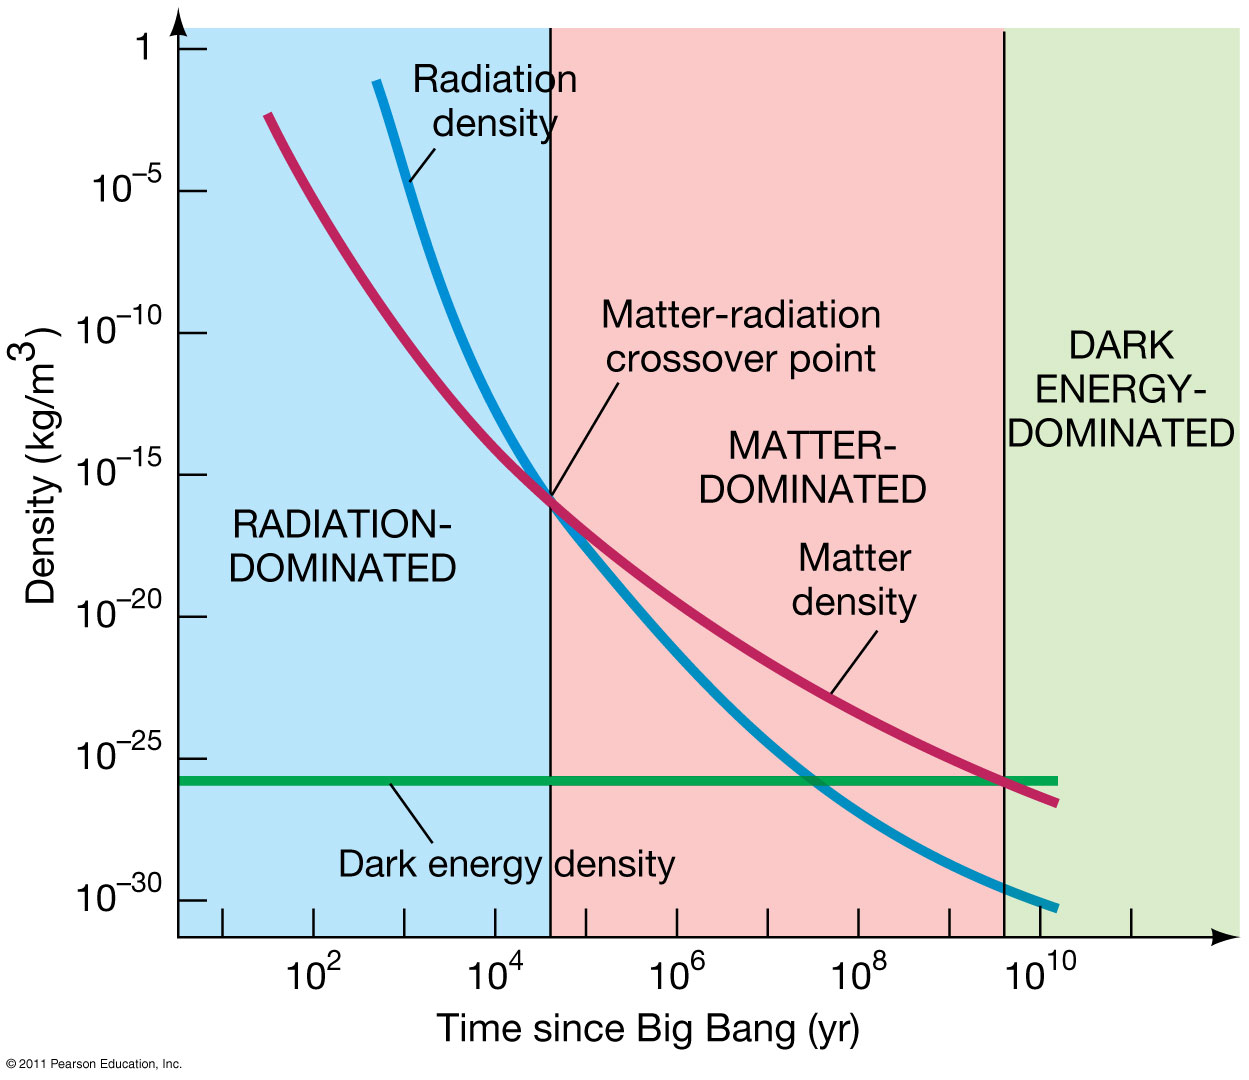
\includegraphics[width=0.55\textwidth]{Kosmo/img/density.jpg}
	\caption{Densitet af hver komponent af universet som funktion af tid. Bemærk at akserne er logaritmiske. Kilde:~\cite{brauComponentsUniverse}.}
	\label{kosmo:fig:figDensity}
\end{figure}
%Billede fra http://pages.uoregon.edu/jimbrau/BrauImNew/Chap27/7th/AT\_7e\_Figure\_27\_01.jpg

Det ville være en dårlig model til data at antage, at universet kun bestod af én ting. Så lad os hellere bruge Benchmark-modellen, hvor alle tre komponenter, beskrevet her, indgår.
Kigger vi på \cref{kosmo:eq:friedmann_component}, så ser det ud til, at stråling og stof må have spillet en større rolle i universets barndom, end det gør i dag. Densiteten var højere (da $a$ var lille) og det udgjorde en større andel af den samlede densitet, når vi husker på, at mængden af kosmologisk konstant per. rummængde er konstant. Selvom energien fra stråling er meget lav i dag, så falder den også hurtigst, og det betyder, at den engang har været dominerende (utroligt høj strålingsdensitet) i universet. Der skal vi selvfølgelig meget langt tilbage. Helt til universet kun var $47$ tusind år gammelt. Den kosmologiske konstant har domineret siden universet var $9.8\,\text{mia. år}$ gammelt, og i dag er det $13.8\,\text{mia. år}$. Det er altså relativt kort tid (kun godt $4\,\text{mia. år}$) siden  mørk energi begyndte at dominere. De forskellige perioder og densiteter er indtegnet på \cref{kosmo:fig:figDensity}.
Vi kan lave en approksimation og antage, at i hver fase vil skalafaktoren $a$ udvikle sig, som om universet kun består af den komponent, der dominerer.

Udover disse faser, skete der en voldsom inflation lige i starten omkring $\SI{e-35}{}-\SI{e-32}{\second}$ efter Big Bang. I løbet af dette tidsrum blev universet $\num{e26}$ gange større. Det gik fra at være på størrelse med en proton til ca. en grapefrugt. Drivkraften menes at have været en anden form for kosmologisk konstant, der dominerede netop der, men senere blev overgået af stråling og stof. Massen fik så universets udvidelse til at deccelerere igen, indtil den kosmologiske konstant for nylig overtog. Baggrunden for denne teori er, at den forklarer hvorfor universet er så fladt (ujævnheder blev udjævnet), og hvorfor temperaturen er så ens overalt i det synlige univers. Man skulle tro, at hvis hver ende af det synlige univers aldrig ville have været i kontakt, så de ville ikke kunne udveksle energi. I det tilfælde vil der ikke være grund til at de skulle have samme temperatur. Alligevel er temperaturfordelingen i baggrundsstrålingen som samme sortlegeme (se \cref{kosmo:fig:cmbplanck}) overalt på Himlen. Det betyder, at baggrundsstrålingen er varmestråling med samme temperatur overalt. Hvis alt lå virkelig tæt før inflationen, så kunne informationer og varme godt udveksles førhen. Det er altså en forklaring på, hvorfor det kosmologiske princip gælder i det synlige univers.
%\section{Universets skæbne}

\begin{figure}[]
    \centering
    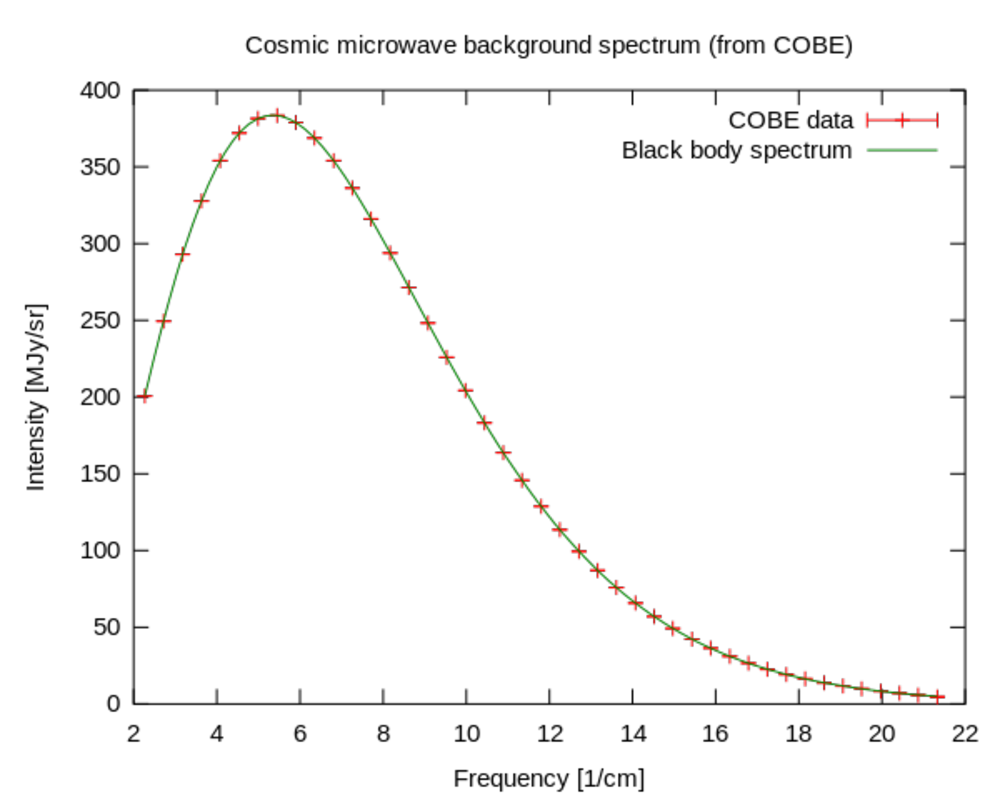
\includegraphics[width = .6\textwidth]{Kosmo/img/cmbplanck.pdf}
    \caption{Et plot af målinger af baggrundsstrålingens frekvensspektrum med eksperimentet COBE, sammenlignet med et teoretisk sort-legeme spektrum for et objekt med samme temperatur. Variationen (samt usikkerhed) fra det forventede er lavere, end man kan plotte, selv med en forstørrelse af grafen. Kilde:~\cite{CosmicMicrowaveBackground}.}
    \label{kosmo:fig:cmbplanck}
\end{figure}

\section{Mørkt Stof} \label{kosmo:sec:DM}
%Noget med rotationskurver af galakser, v af galakser i hobe, gravitational lensing

Ikke alene er det meste af det massen fra stof udetekterbart for vores øjne, men det er ikke nødvendigvis baryonisk heller. Størstedelen af stoffet i universet er ikke-baryonisk mørkt stof, hvilket betyder, at det ikke vekselvirker med den elektromagnetiske kraft, og derved hverken absorberer, emitterer eller spreder lys ved nogen bølgelængde. En måde hvorpå mørkt stof kan detekteres, er ved at se på dets gravitationelle indflydelse på synligt stof. En klassisk metode er at se på omløbshastigheden af stjerner i spiralgalakser. Mælkevejen er f.eks. en spiralgalakse. Tag nu Solen. Den er i en afstand $R=\SI{8.5}{\kilo\parsec}$ fra centrum af galaksen, og har en omløbshastighed på omkring $v=\SI{220}{\kilo\meter\per\second}$. Solen vil opleve en centripetalacceleration
%
\begin{align}
    \ddot{x} &= \frac{v^2}{R}
    %
    \intertext{mod centrum af galaksen. % Undersøg, hvorvidt følgende tekststykke stadig giver mening i år
    Hvis accelerationen $\ddot{x}$ er givet ved gravitationel tiltrækning\footnote{Newtons universelle tyngdelov har samme afstandsafhængighed som Coulombs lov. Man kan således definere et tyngdefelt, der opfylder en version af Gauss' lov, se \cref{sec:gauss}, og dermed vise at \cref{eq:gravitationel_gauss} er sand.}, så er}
    %
    \ddot{x} &= \frac{G M(R)}{R^2}, \label{eq:gravitationel_gauss}
    %
    \intertext{hvor $M(R)$ er massen af galaksen indenfor en bestemt radius, $R$. De to ovenstående ligninger kan vi sætte lig hinanden, og derved få et udtryk for hastigheden:}
    %
    \frac{v^2}{R} &= \frac{G M(R)}{R^2}
    %
    \intertext{eller}
    %
    v &= \sqrt{\frac{G M(R)}{R}}. \label{kosmo:eq:fart_i_galakse}
    %
    \intertext{Vi kan måle hastigheden af stjerner i en galakse ved hjælp af deres rødforskydning fra Dopplereffekten. Nu ved vi, at hastigheden er højere, desto større en masse stjernen kredser om. Altså kan vi beregne fordelingen af masse, ved at kigge på stjerner forskellige steder i galaksen. Overfladelysstyrken, $I$, af disken i en spiralgalakse aftager med radius (det er den lysstyrke man ser, hvis man kigger på et område af galaksedisken ovenfra). Lysstyrken fortæller, os hvordan stjernerne, dvs. synligt stof, er fordelt. Lyset intensitet\footnote{For en udførlig introduktion til begrebet intensitet af lys se \cref{laser:sec:intensitet}.} kan beskrives som}
    %
    I(R) &= I(0) e^{-R/R_\textup{s}},
\end{align}
%
hvor $R_\textup{s}$ er skalalængden (også kaldt den karakteristiske længde), som typisk ligger indenfor et par kiloparsec. $R_\textup{s}$ er den afstand, hvor $I$ er faldet med en faktor $e$. Vores galakse har $R_\textup{s}\approx \SI{4}{\kilo\parsec}$. Et par skalalængder væk fra centrum af en spiralgalakse begynder massen af stjernerne indenfor $R$ af være konstant -- længere ude er der nemlig næsten intet lys. Hvis stjernerne bidrog til alt eller det meste af massen i en galakse, ville hastigheden falde af som $v \propto 1/\sqrt{R}$ ved store radier, fordi den indesluttede masse ville være nogenlunde konstant. Men det ser vi ikke. Hastighederne holder sig nogenlunde konstante, som på \cref{kosmo:fig:rotationskurve}, så der mangler noget masse. Faktisk mangler der mere masse, jo længere vi bevæger os ud (til en hvis grænse). Denne manglende masse kalder vi mørkt stof, da den ikke er synlig. At den ligger så langt ude er et tegn på, at massen ikke vekselvirker meget med hverken sig selv eller synligt stof, det er energitab fra vekselvirkninger med andre partikler, der får stof til at `falde' ind mod centrum af galaksen. Derfor ligger det mørke stof stadig langt væk fra centrum, hvor det opretholder høje hastigheder. Det mørke stof vekselvirker dog gennem tyngdekraften, så det bliver stadig samlet i galaksers tyngdefelter. Denne komponent af galakser kalder vi haloer af mørk stof (engelsk: dark matter halos). De er sfæriske og ligger altså ikke kun i spiralgalaksens disk.

\begin{figure}[]
	\centering
	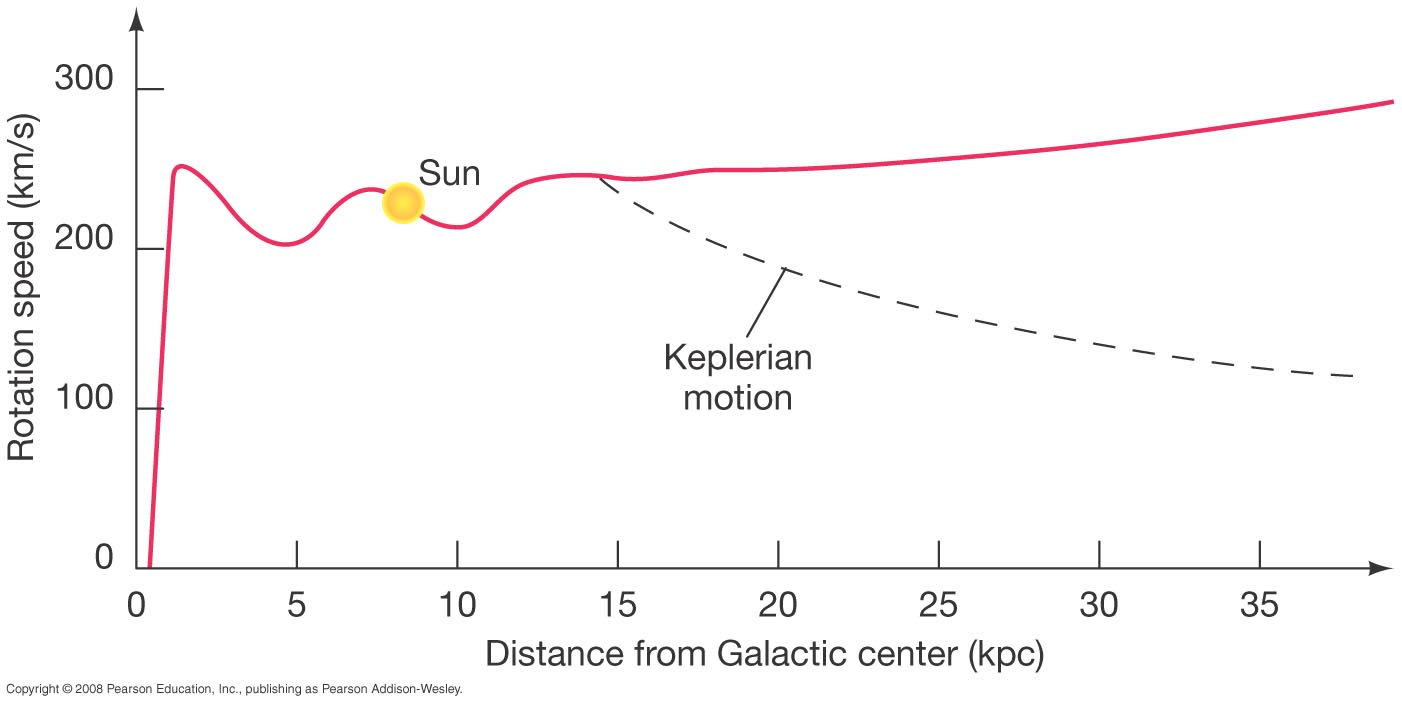
\includegraphics[width=0.65\textwidth]{Kosmo/img/rotationskurve.jpg}
	\caption{Rotationskurve over Mælkevejen. Den solide kurve viser de observerede hastigheder, og den stiplede viser de forventede fra fordelingen af synligt stof. Afstanden mellem kurverne viser fordelingen af mørkt stof. Kilde:~\cite{brauRotationMilkyWay}.}
	\label{kosmo:fig:rotationskurve}
\end{figure}
%Billede fra http://pages.uoregon.edu/jimbrau/BrauImNew/Chap23/6th/23\_21Figure-F.jpg

Man plejede at have to teorier for, hvad mørkt stof består af -- WIMPs og MACHOs. WIMP står for Weakly Interacting Massive Particles og ville være en ny, tung type elementarpartikler. MACHO står for Massive Compact Halo Objects og er mere almindelige ting, såsom sorte huller, svage dværgstjerner og `forældreløse' planeter, der er blevet slynget væk fra deres stjerner. Ting, der ikke lyser nok til, vi ville kunne se dem på lang afstand. Man har nu udelukket, at MACHOs kan udgøre en signifikant del af det mørke stof, da vi ville kunne se dets klumper af tyngdekraft deformere lyset af objekter bagved. Dette fænomen, kaldet \emph{gravitationslinseeffekten}, ses dog i mange andre sammenhænge f.eks. fra det mørke stof af en hel galakse. 

\iffalse
\subsection{Gravitationelle Linser}

En af konsekvenserne af generel relativitetsteori er, at et massivt objekt kan fungere som en linse, der bøjer lyset fra en fjernere kilde. F.eks. kan lyset fra et astronomisk objekt blive bøjet af tyngdefeltet fra en større mængde af masse (normalt samlet i galakser), der ligger mellem kilden og observatøren. Jo mere massiv en genstand er, desto større en linseeffekt ser vi. Derfor kan vi fra effekten regne os frem til massen af det mellemliggende objekt. Hvis det er en galakse, kan vi se, at den bøjer rummet meget mere end hvad den burde ud fra det synlige lys. Igen mangler der altså masse, og mørkt stof må eksistere.


Stærk lensing er når forvrængningen af f.eks. baggrundsgalakser, danner flere billeder af den samme galakse eller en hel ring rundt om det tunge objekt (også kaldet en Einstein ring). Dette har vi observeret omkring mange fjerne hobe, hvilket inkluderer den berømte Abell 1689, se \cref{kosmo:fig:abell1689}. Ved måling af forvrængningsgeometrien (engelsk: distortion geometry) kan massen af den mellemliggende hob findes. %I mange tilfælde, hvor man har gjort dette, opnåede man masse-til-lys forhold svarende til det dynamiske mørke stof målt i hoben.

Svag gravitationel lensing undersøger små forvrængninger ved hjælp af statistiske analyser fra store galakseundersøgelser. Ved at undersøge den tilsyneladende forskydningsdeformation af de tilstødende baggrundsgalakser, kan den gennemsnitlige fordeling af mørk stof karakteriseres.

Gravitationslinseeffekten kan også bruges til at opdage exoplaneter (planeter uden for Solsystemet). Det gælder, hvis lyset fra et objekt passerer en stjerne med en exoplanet, før det når frem til os. Så vil linsen forstærke lyset, og vi ser et ekstra lille bump fra planetens tyngdekraft.

\begin{figure}[H]
	\centering
	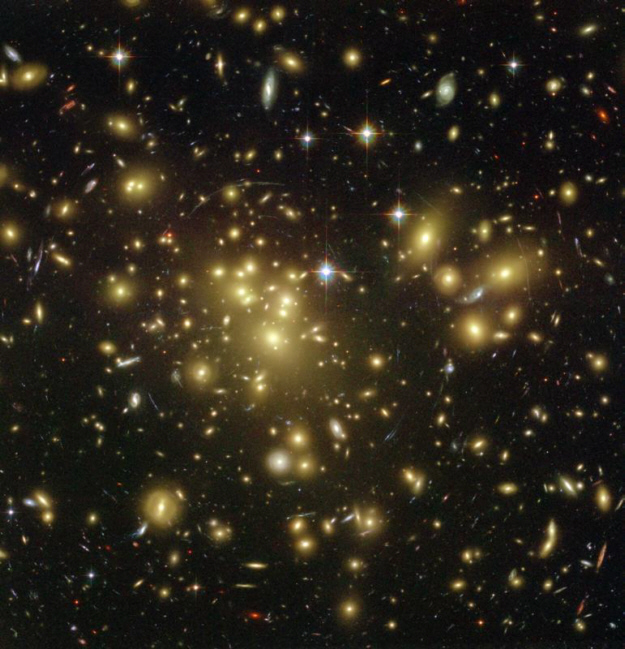
\includegraphics[width=0.6\textwidth]{Kosmo/img/abell1689.jpg}
	\caption{Stærk gravitationel lensing observeret med Hubble Space Telescope, hvilket er en indikator for mørkt stof. Billede fra Hubble Space Telescope.}
	\label{kosmo:fig:abell1689}
\end{figure}
\fi

\section{Afstande og Luminositet}
Afstand er et vigtigt begreb i astrofysikken og kosmologien, men ofte også svært at måle. Derfor har vi mange forskellige typer afstandsmål, og hvordan de hænger sammen, er ikke altid fastlagt. En af de mest brugte metoder til bestemmelse af afstande er gennem et objekts \textit{luminositet}. Et objekts absolutte luminositet, $L$, er defineret som den energi, der er udsendt per tid. Det har vist sig, at en stjernes luminositet, hvis vi antager, at det er et sortlegeme, er relateret til dets radius $R$ og temperatur $T$:
%
\begin{align}
    L &= 4\pi\sigma R^2T^4 \propto R^2 T^4
\end{align}
%
hvor $\sigma$ er Stefan-Boltzmann's konstant. Hvis denne energi er udsendt uniformt i alle retninger og modtages i en afstand $d_L$ væk, er den modtagede \emph{tilsyneladende luminositet}, eller \emph{flux}, givet ved:
%
\begin{align}
    F &= \frac{L}{4\pi d_L^2}, \label{kosmo:eq:flux}
    %
    \intertext{hvor $d_L$ er luminositetsafstanden.\endgraf
    Et andet eksempel på et afstandsmål, er vinkelafstanden. Her kigger man simpelthen på hvor stor en vinkel, $\Delta \theta$, objektet udspænder på himlen. Metoden kræver adgang til en standardlineal, dvs. et objekt hvis \emph{egenlængde}, $l$, er kendt. Egenlængden er den længde, man ville måle med en lineal fra den ene til den anden side, hvis man kunne komme tæt på. Standardlinealen skal være bundet godt sammen af enten tyngdekraften, gaffatape, eller måske en helt tredje kraft, som ikke tillader objektet at ekspandere med universet. Vinkelafstanden, $d_\textup{A}$, opskrives som}
    %
	d_\textup{A} &= \frac{l}{\Delta \theta}.
	%
    \intertext{For eksempel kan det antages, at galaksernes størrelse er fast i tid, og $l$ kan så være galaksernes faste størrelse, uafhængigt af afstanden til galaksen.
    Udtrykkene for disse afstande er dog mest praktiske, når de er skrevet som funktion af $z$, da rødforskydningen altid er observerbar. De kan let blive skrevet som en funktion af skalafaktoren, $a$, samt andre parametre, ved at lave små og forholdsvis simple transformationer. For eksempel er de to udtryk for $d_L$ og $d_\textup{A}$ næsten ens, men med en lille forskel:}
    %
    d_L(z) &= (1+z)d_\textup{M}(z), \\
    d_\textup{A}(z) &=\frac{d_\textup{M}(z)}{1+z},
\end{align}
%
hvor $d_\textup{M}(z)$ afhænger af krumningen af universet. $d_\textup{M}(z)$ kaldes på engelsk ``transverse comoving distance'', men lad os her blot betragte det som en faktor til at relatere rødforskydningen til andre afstandsmål.

Indenfor astronomiens verden beskrives et objekts lysstyrke ved \emph{magnitudesystemet}. Dette er et logaritmisk system, der rækker helt tilbage til Hipparchos i antikkens Grækenland. Af historiske årsager fungerer systemet således, at jo højere magnituden bliver, desto svagere ser objektet ud på himlen og omvendt. Dengang fandtes der ikke teleskoper, som i dag, så alle målinger af stjerner blev taget per øjemål. Dengang gik skalaen fra 0 til og med 6, hvor 0 var det stærkeste på himlen og så fremdeles. Vi bruger i dag en skala, der er defineret således, at grækernes målinger stadig passer ind. Den tilsyneladende magnitude af et objekt vil variere med afstanden -- hvis man flytter sig tættere på en stjerne, vil den få en lavere magnitude (svarende til højere lysstyrke). Hvis man tager højde for afstanden, får man objektets absolutte magnitude, der er ens for alle observatører.

\subsection{Standardlyskilder}

En standardlyskilde (engelsk: standard candle) er et astronomisk objekt, der har en kendt absolut magnitude. Disse er supervigtige for astronomer, da man, ved hjælp af den tilsyneladende magnitude af et objekt, kan bestemme afstanden ved at bruge
%
\begin{align}
    m-M=5\cdot \log_{10}\left(\frac{d_L}{[\textup{pc}]}\right) - 5 ,
\end{align}
%
hvor $m$ er den tilsyneladende magnitude, $M$ er den absolutte magnitude, og $d_L$ er afstanden til objektet målt i parsec ([pc]). Forskellen kaldes objektets distancemodulus. Når der divideres med parsec, så er det blot for at fjerne længdeenheden, da man kun kan tage logaritmen til et tal uden enhed.

To af de mest anvendte standardlyskilder indenfor astronomi er Cepheide-variable stjerner og RR-Lyræ-stjerner. I begge tilfælde kan stjernernes absolutte magnituder bestemmes ud fra deres variabilitetsperioder. Med variable stjerner menes stjerner, hvis lysstyrke (eller tilsyneladende magnitude, set fra Jorden) ændrer sig over tid. Dette kan enten være grundet ændringer i stjernens luminositet/faktiske lysudsendelse (intrinsisk variable stjerner), eller ændringer i lyset efter udsendelse, for eksempel hvis det blokeres på vej mod os (ekstrinsiske variable stjerner). Cepheide-variable stjerner og RR-lyræ-stjerner er typer af intrinsisk variable stjerner. 

En nyere tilføjelse til gruppen af standardlyskilder er Type Ia supernovaer. Disse kan også klassificeres som standardlyskilder, men er i virkeligheden standardiserbare lyskilder, da de ikke har præcist den samme maksimale lysstyrke. Forskellene i deres maksimale lysstyrke hænger dog sammen med, hvor hurtigt lyskurven aftager efter maksimal lysstyrke. Her ser man på forskellem mellem den maksimale lysstyrke og lysstyrken 15 dage efter. Dette kaldes også $\Delta m_{15}$. Hvis denne har en værdi mindre end $1$ er objektet lysstærkt, mens den ved en værdi over $1$ er lyssvagt.

\subsection{Olbers paradoks}
Lad os undersøge et simpelt spørgsmål: hvorfor er nattehimlen mørk? Eller rettere: hvorfor er den ikke uendeligt lys? Hvis vi lever i et uendeligt univers med en homogen og isotrop fordeling af stjerner, hvorfor ser vi så ikke uendeligt mange stjerner på himlen?

Vi kan opstille en formel for, hvor meget lys vi modtager. Mængden af modtaget lys må stige med antalsdensiteten af stjerner (antallet af stjerner per volumen) $n$, falde med afstanden fra os observatører, kaldet $r$, og stige med den flux af fotoner vi modtager fra hver stjerne, som vi kalder for $F$. Vi ønsker at finde intensiteten, $I$, som er den flux, vi modtager per areal (hvor vi observerer) per rumvinkel på himlen. Dette er hvad vi rent fysisk forventer.

Den søgte formel kan vi finde, hvis vi grupperer alle stjerner efter, hvor langt de er fra os. Dette gøres ved at betragte alle stjerne med en bestemt afstand, $r$, til os som værende på en kugleskal % Vi kan summe bidragene fra alle kugleskalle af stjerner, hvor hver skal har en 
med tykkelse $\dd{r}$. Det lille bidrag til den samlede intensitet, $\dd{I}$, er den mængde lys, vi modtager fra hver stjerne, $F$, gange det antal stjerner, der er på kugleskallen, $N$. Antallet af stjerner på kugleskallen er antalstætheden, $n$, gange volumen af kugleskallen, $V_\mathrm{skal} = 4\pi r^2 \dd{r}$. Dermed bidrager kugleskallen med intensiteten
%
\begin{align}
	\dd{I} = FN = F n4\pi r^2\dd{r}. %Hvorfor ikke 4pir^2?
\end{align}
%
Her kan vi indsætte udtrykket for $F$ fra afstandskvadratloven i \cref{kosmo:eq:flux}, hvor afstanden $d_L = r$: %Tjek at vi har nævnt den først
%
\begin{align}
	\dd{I} = \frac{L}{4\pi r^2} 4\pi nr^2\dd{r} = L n \dd{r}. 
\end{align}
%
For at finde den totale intensitet, betragter vi hver skal som værende infinitesimalt tynd, og integrerer over hele det uendelige univers:
%
\begin{align}
	I =\int^\infty_0 Ln \dd{r}.
\end{align}
%
Her er en masse konstanter, der ikke vil ændre sig som funktion af radius, så dem kan vi trække ud af integralet
%
\begin{align}
	I = Ln \int^\infty_0 \dd{r} = L n \big[r\big]_0^\infty = L n \big(\infty - 0\big) = \infty.
\end{align}
%
Ergo må universet være uendelig lyst. Dette holder som bekendt ikke i virkeligheden, da der faktisk ligger en del antagelser bag udledningen. Brug gerne et øjeblik til at overveje, hvad du tror årsagen er.
%
\begin{itemize}
    \item Det kunne f. eks. være universet ikke er homogent, så der kun findes stjerner tæt på os, eller dem langt væk lyser mindre. Det har vi dog ingen anden grund til at tro er tilfældet. Men hvis $nL \propto 1/r^x$, for $x>1$, så kan himlen være mørk.
    \item Det kunne også være universets krumning betyder, at vi ikke kan bruge afstandskvadratloven, så fluxen falder hurtigere med afstand. Det ser vi dog ingen tegn på indtil videre.
    \item En tredje antagelse, er at vi kan se alle stjerner, uden andre objekter kommer i vejen for vores synslinjer. Hvis stjernerne skygger for hinanden, så bliver himmelen ikke uendeligt lys, men får en jævn lysstyrke som overfladen på en stjerne, hvilket stadig ikke giver en mørk himmel. Andet materiale kunne også skygge for stjernerne, men det ville i så fald absorbere lys, indtil det udsender lige så meget energi, som det absorberer. Det vil sige, at det også ville lyse lige så kraftigt som stjernerne, hvorfor det heller ikke løser problemet.
    \item Det kan være, at universet ikke er uendelig stort, så der ikke er nogen stjerner efter en hvis radius.
    \item Hvis universet udvider sig så hurtigt, at stjerners lys rødforskydes nok til vi ikke kan opfange det, så vil det også gøre himlen mørk.
\end{itemize}
%
Den primære løsning til Olbers paradoks er dog, at universet ikke er uendeligt gammelt. Det betyder, at lyset fra fjerne stjerner simpelthen ikke er nået frem til os endnu.

% Vi kan opstille en formel for hvor meget lys vi modtager. Det må stige med antalsdensiteten af stjerner (stjerner per volumen) $n$, falde med afstanden fra os observatører, kaldet $r$, og stige med den flux af fotoner vi modtager fra hver stjerne, som vi kalder for $F$. Vi ønsker at finde intensiteten, $I$, som er den flux vi modtager per areal (hvor vi observerer) per rumvinkel på himlen.

% Det kan vi finde, hvis vi grupperer alle stjerner efter hvor langt de er fra os. Vi kan summe bidragene fra alle kugleskalle af stjerner, hvor hver skal har en tykkelse $\dd r$. Det lille bidrag til den samlede intensitet er da
% \begin{align}
% 	\dd I = Fnr^2\dd r %Hvorfor ikke 4pir^2?
% \end{align}
% Her kan vi indsætte udtrykket for $F$ fra afstandskvadratloven \ref{eq:L} %Tjek at vi har nævnt den først
% \begin{align}
% 	\dd I = \frac{L}{4\pi r^2} nr^2\dd r = \frac{L}{4\pi} n \dd r. 
% \end{align}
% For at finde summen af alle bidragene fra kugleskallerne, gør vi hver skal infinitesimalt tynd og integrerer over hele det uendelige univers:
% \begin{align}
% 	I =\int^\infty_0 \frac{L}{4\pi r^2} nr^2 \dd{r}
% \end{align}
% Her er en masse konstanter, der ikke vil ændre sig som funktion af radius, så dem kan vi trække ud af integralet
% \begin{align}
% 	I =\frac{L}{4\pi r^2} n \int^\infty_0 r^2 \dd{r} =\frac{L}{4\pi r^2} n \cdot \infty = \infty
% \end{align}
% Ergo må universet være uendeligt lyst.  Dette holder som bekendt ikke i virkeligheden, da der faktisk ligger en del antagelser bag udledningen.


\end{document}